\subsection{Troposphere: Scottish Highlands, GFS refractivity}
The path runs from \ang{57.2163}N \ang{4.9214}W (top of a \SI{664}{m} ridge) to
\ang{57.40}N \ang{4.60}W (\SI{28}{km}). The data are:
\begin{itemize}
\item elevation tiles of \texttt{pywaveprop.environment} at \ang{0.0005} resolution
(terrain from 166 to \SI{664}{m}, smoothed with $\sigma=\SI{100}{m}$, maximum slope
$11.1^\circ$);
\item the modified refractivity of the GFS analysis 2026-10-09T12:00Z interpolated
along the path and averaged over range (\cref{fig:tropo}, right).
\end{itemize}
A \SI{300}{MHz} H-polarised antenna on a \SI{30}{m} mast (beam $4^\circ$, tilted
$1^\circ$ down) radiates over perfectly conducting ground. The aperture is
$5^\circ+2\cdot11.1^\circ=27.3^\circ$
(\cref{cor:angles}) for both solvers, and the staircase solver sees the same
smoothed terrain.
Path loss \SI{10}{m} above the ground (median / 90th percentile of the difference):
\begin{itemize}
\item the two precision settings of the terrain-following solver differ by
0.08 / 0.17\,dB;
\item those of the staircase solver differ by 0.15 / 0.48\,dB;
\item the two solvers at the finer setting differ by 1.09 /
3.04\,dB (at \SI{50}{m}: 0.44 / 1.35\,dB).
\end{itemize}
Each solver is thus converged with respect to its own grid; the two agree to
about \\SI{1}{dB} (median) \\SI{10}{m} above the ground and \\SI{0.4}{dB} at
\\SI{50}{m}. The largest differences, up to a few
decibels, occur on the slopes facing the transmitter (21--23\,km and the first
kilometres). There the staircase solution carries small-scale ripple that the
smooth-boundary solution does not, consistent with scattering by the steps
(\cref{sec:slope}).
Run times: terrain-following 468 and 1390\,s,
staircase 73 and 117\,s.
\begin{figure}[t]\centering
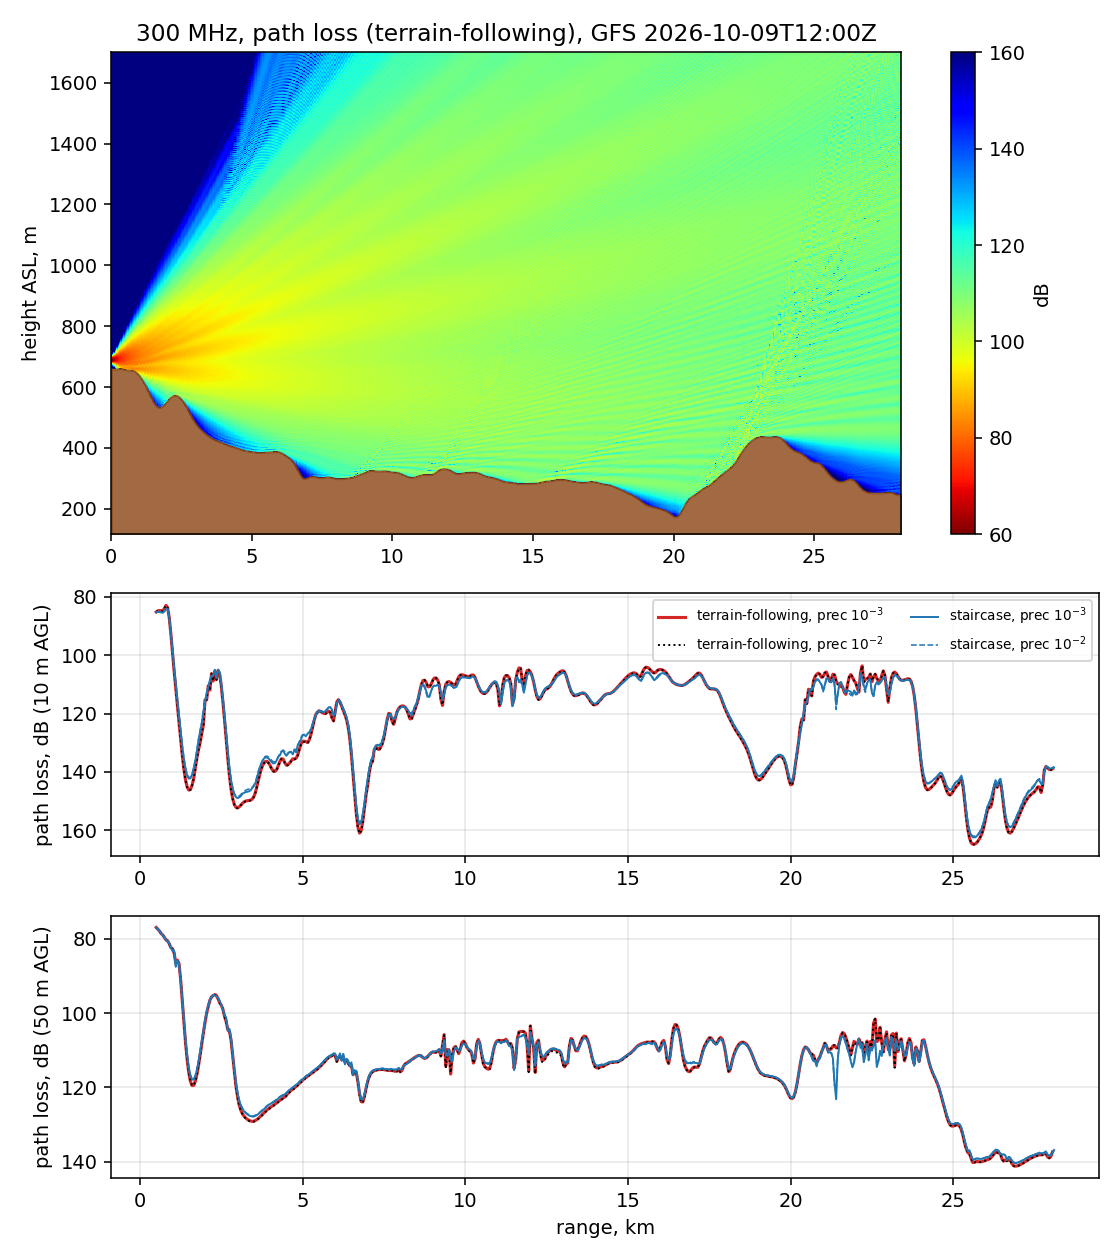
\includegraphics[width=0.74\textwidth]{troposphere_highlands.png}\hfill
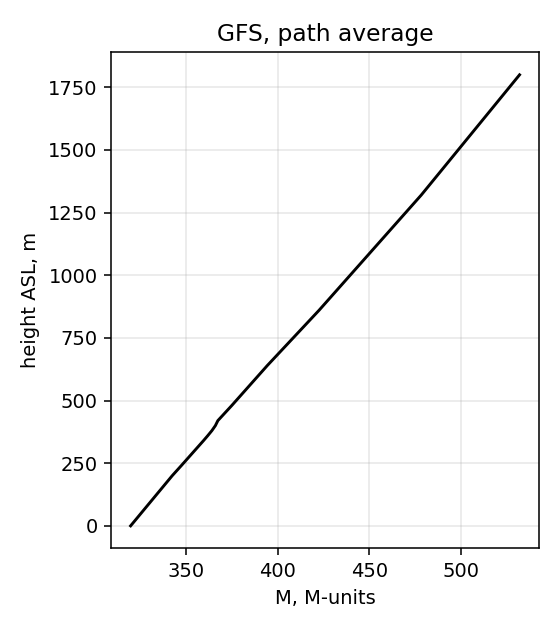
\includegraphics[width=0.25\textwidth]{troposphere_highlands_M.png}
\caption{Scottish Highlands, \SI{300}{MHz}. Path loss of the terrain-following
solver (top), path loss \SI{10}{m} and \SI{50}{m} above the ground for both solvers
and two precision settings, and the GFS M-profile.}\label{fig:tropo}
\end{figure}
\subsection{Underwater acoustics: Bermuda pedestal, Argo sound speed}
The path runs from \ang{32.475}N \ang{64.598}W (\SI{100}{m} deep, on the
edge of the Bermuda platform) to \ang{32.70}N \ang{64.40}W (\SI{3400}{m}).
The data are:
\begin{itemize}
\item bathymetry from the elevation tiles at \ang{0.002} (smoothed with
$\sigma=\SI{500}{m}$, maximum slope $16.1^\circ$);
\item the mean Argo sound speed profile of the area (2020--2023) to \SI{2000}{m},
extended with the deep isothermal gradient \SI{0.0165}{s^{-1}};
\item a fluid bottom (\SI{1700}{m/s}, 1.5, \SI{0.5}{dB/\lambda}) whose interface
follows the bathymetry.
\end{itemize}
A \SI{100}{Hz} source \SI{50}{m} deep radiates down the slope. All solvers start
from RAM's self-starter. The terrain-following domain extends to
\SI{9063}{m}, and the NLBC lies in the homogeneous bottom. The
reference is double-precision RAM at $\Delta r=\SI{2.5}{m}$,
$\Delta z=\SI{0.125}{m}$; RAM at $(5, 0.25)$\,m differs from it by
0.11--0.14\,dB (median).
\begin{table}[h]\centering
\caption{Bermuda pedestal: median / 90th percentile of $|\Delta\mathrm{TL}|$ (dB) with
respect to RAM ($\Delta r=2.5$, $\Delta z=0.125$\,m), $r>\SI{500}{m}$.}\label{tab:bermuda}
\begin{tabular}{llcc}\toprule
aperture & solver (grid) & $z=\SI{50}{m}$ & $z=\SI{500}{m}$\\\midrule
$70^\circ$ & terrain-following ($\Delta x=5.0$, $\Delta z=0.29$\,m) & 0.68 / 2.04 & 0.74 / 4.54\\
$70^\circ$ & stair-step ($\Delta x=5.0$, $\Delta z=0.67$\,m) & 0.42 / 0.89 & 0.59 / 2.86\\
-- & RAM ($\Delta r=5$, $\Delta z=0.25$\,m) & 0.11 / 0.40 & 0.14 / 1.04\\
\bottomrule\end{tabular}\end{table}
\begin{figure}[t]\centering
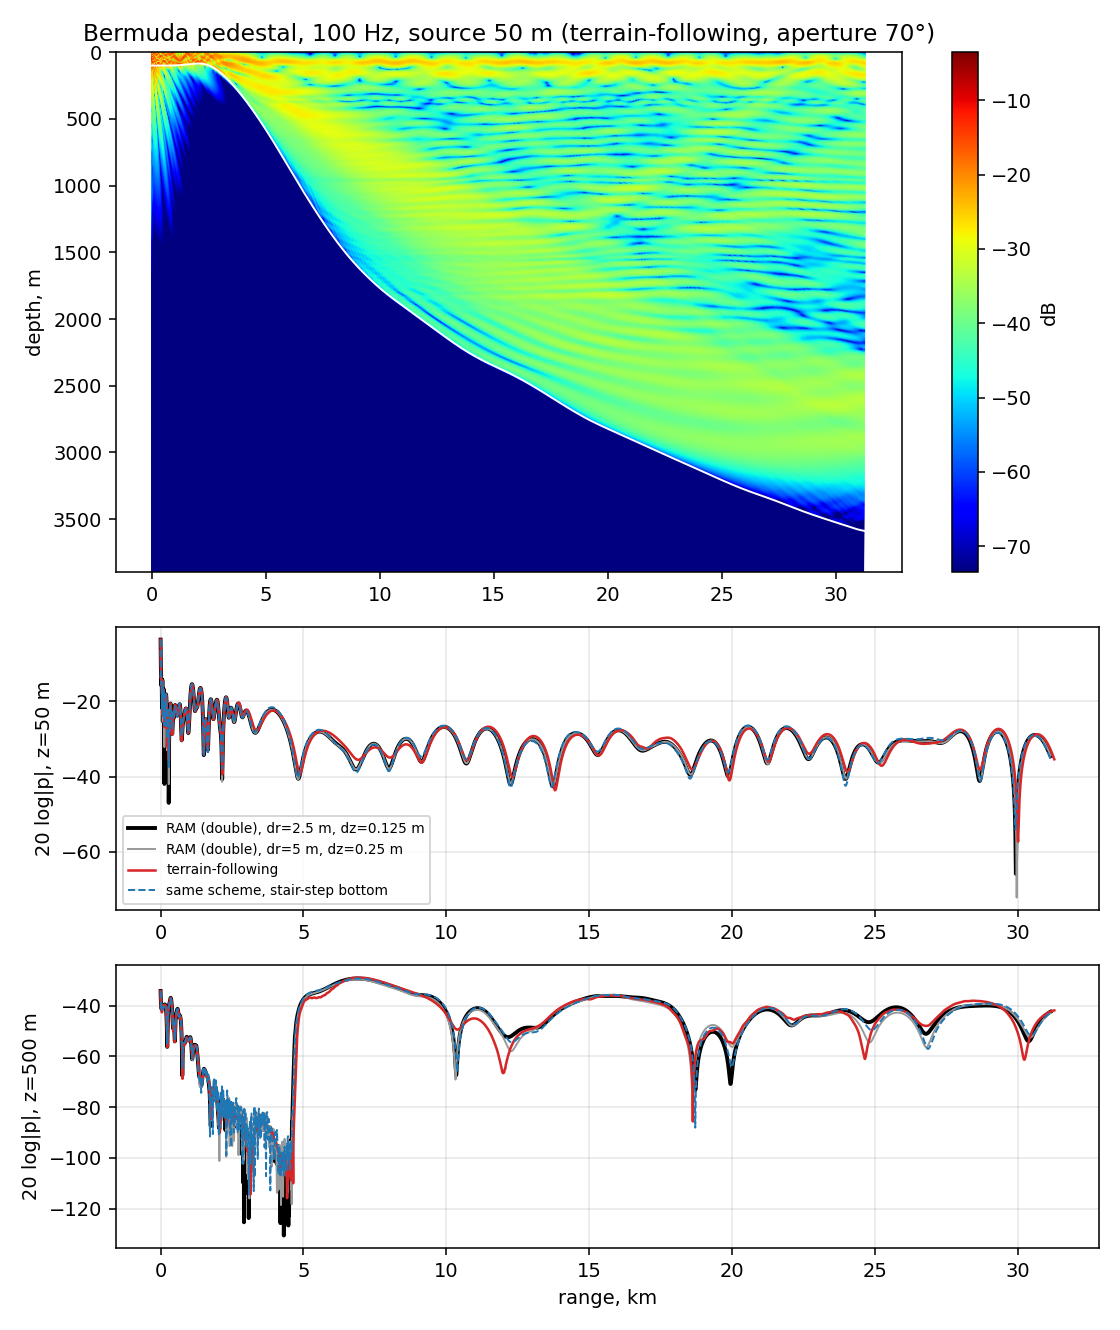
\includegraphics[width=0.8\textwidth]{underwater_bermuda_70deg.png}
\caption{Bermuda pedestal, \SI{100}{Hz}: field of the terrain-following solver
($70^\circ$ aperture) and $20\log|p|$ at \SI{50}{m} and \SI{500}{m} depth.}\label{fig:bermuda}
\end{figure}
With a $70^\circ$ aperture (\cref{tab:bermuda}, \cref{fig:bermuda}) the
terrain-following solution differs from the RAM reference by
0.68 and 0.74\,dB (median at 50 and
\SI{500}{m}); the stair-step bottom gives 0.42 and
0.59\,dB.

The difference is not a discretisation error:
\begin{itemize}
\item halving $\Delta x$ changes it by \SI{0.03}{dB} (0.69/0.74 $\to$ 0.65/0.71\,dB);
\item raising the flux order to $q=3$ changes it by less than \SI{0.02}{dB} (0.66/0.70\,dB);
\item lowering $\etab$ from \SI{3600}{m} to \SI{1200}{m} reduces it to 0.54/0.65\,dB.
\end{itemize}
With $\etab=\max T$ the $\sigma$-map compresses the \SI{100}{m} shelf column 36 times, so $r$ jumps by a factor of about 30 across the seabed. Part of the
difference is therefore the second-order treatment of this extreme interface
row, and a less compressive choice of $\etab$ is preferable for large depth
contrasts. The remainder is of the same order as the difference between the two
stair-step solvers (ours and RAM). Over a \ang{16} penetrable slope, RAM is
itself a stair-step one-way model, and we have no exact reference to say which
one-way treatment is closer to the full solution. The exact test of
\cref{sec:slope} and the wedge of \cref{tab:wedge} are the discriminating
cases.
Times: terrain-following 273\,s, stair-step 966\,s, RAM
27\,s and 97\,s.
